\documentclass[10pt,a4paper,oneside]{article}
\usepackage[utf8]{inputenc}
\usepackage{amsmath}
\usepackage{amsfonts}
\usepackage{amssymb}
\usepackage{graphicx}
\usepackage{breqn}
\usepackage{draftwatermark} % 设置水印
\SetWatermarkText{DNV Group} % 水印内容
\usepackage{tikz} % system block diagram
\usepackage{textcomp}
\usetikzlibrary{datavisualization}
\usetikzlibrary{shapes,arrows} % system block diagram
\usepackage{booktabs}
\usepackage[framed,numbered,autolinebreaks,useliterate]{mcode} % matlab code block
\author{Yangang Cao}
\date{February 27, 2019}
\newcommand{\degree}{^\circ}
\tikzset{
	delay/.style    = {draw, thick, rectangle, minimum height = 3em,
		minimum width = 3em},
	sum/.style      = {draw, circle, node distance = 2cm}, 
	prod/.style     = {draw, circle, node distance = 2cm},
	input/.style    = {coordinate}, % Input
	output/.style  = {coordinate} % Output
}
% Defining string as labels of certain blocks.
\newcommand{\product}{$\displaystyle \times$}
\newcommand{\delay}{\large$z^{-1}$}
\begin{document}

\title{Noise Gate}
\maketitle 
A noise gate can be considered as an extreme expander with a slope of −$\infty$. This results in the complete muting of signals below the chosen threshold $NT$. As the name implies, the noise gate is typically used to gate out noise by setting the threshold just above the level of the background noise, such that the gate only opens when a desired signal with a level above the threshold is present. A particular application is found when recording a drum set. Each element of the drum set has a different decay time. When they are not manually damped, their sounds mix together and the result is no longer distinguishable. When each element is processed by a noise gate, every sound can automatically be faded out after the attack part of the sound. This results in an overall cleaner sound. The functional units of a noise gate are shown in following block diagram.
\begin{center}
	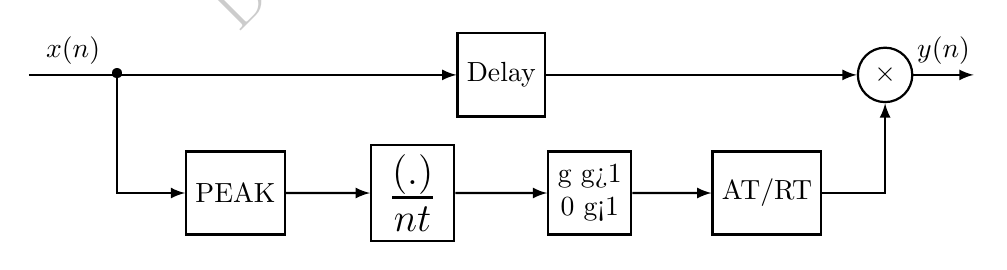
\begin{tikzpicture}[auto, thick, node distance=0.6cm, >=latex, scale = 0.75]
	\draw
	node at (1,0) {\textbullet}
	node at (3,-2) [delay](d1) {PEAK}
	node at (6,-2) [delay] (d2){\huge$\frac{(.)}{nt}$}
	node at (9,-2) [delay,align=center] (d3){g g>1\\0 g<1}
	node at (12,-2) [delay] (d4){AT/RT}
	node at (14,0) [prod] (p1){\product}
	node at (7.5,0) [delay] (d5){Delay};
	
	\draw[-](-0.5,0)--node{$x(n)$}(1,0);
	\draw[->](1,0)|-(d1);
	\draw[->](d1)--(d2);
	\draw[->](d2)--(d3);
	\draw[->](d3)--(d4);
	\draw[->](d4)-|(p1);
	\draw[->](1,0)--(d5);
	\draw[->](d5)--(p1);
	\draw[->](p1)--node{$y(n)$}(15.5,0);
	\end{tikzpicture}
\end{center}
The decision to activate the gate is typically based on a peak measurement which leads to a fade in/fade out of the gain factor with appropriate attack and release times. 
\begin{center}
	\includegraphics[height=130pt]{noisegate.eps} 
\end{center}
Further possible refinements include the use of two thresholds to realize a hysteresis and a hold time to avoid unpleasant effects when the input level fluctuates around the threshold. 
\begin{center}
	\includegraphics[height=250pt]{noisegatehysteresis.eps} 
\end{center}
These are demonstrated in the implementation given in following code.
\begin{lstlisting}
function y=noisegt(audio, para)

% noise gate with hysteresis
% para(1): time in seconds the sound level has to be below the 
%		    threshhold value before the gate is activated
% para(2): threshold value for activating the gate
% para(3): threshold value for deactivating the gate > para(2)
% para(4): time in seconds before the sound level reaches zero
% para(5): time in seconds before the output sound level is the 
%		  same as the input level after deactivating the gate
% para(6): pole placement of the envelope detecting filter < 1
% para(7): sampling frequency

rel = round(para(4)*para(7));  %number of samples for fade 
att = round(para(5)*para(7));   %number of samples for fade 
g = zeros(size(audio));
lthcnt = 0;
uthcnt = 0;
ht = round(para(1)*para(7));
h = filter([(1-para(6))^2], [1.0000 -2*para(6) para(6)^2], abs(audio)); %envelope detection 
h = h / max(h);
for i = 1: length(h)
	if (h(i) <= para(2)) | ((h(i) < para(3)) & (lthcnt > 0)) % Value below the lower threshold?
		lthcnt = lthcnt + 1;		
		uthcnt = 0;
		if lthcnt > ht % Time below the lower threshold longer than the hold time?
			if lthcnt > (rel + ht) 
				g(i) = 0;
			else
				g(i) = 1 - (lthcnt-ht) / rel;		% fades the signal to zero
			end
		elseif ((i < ht) & (lthcnt == i))
			g(i) = 0;
		else
			g(i) = 1;
		end
	elseif (h(i) >= para(3)) | ((h(i) > para(2)) & (uthcnt > 0))	
	% Value above the upper threshold or is the signal being faded in?
		uthcnt = uthcnt + 1;
		if (g(i-1) < 1) % Has the gate been activated or isn't the signal faded in yet?
			g(i) = max(uthcnt/att, g(i-1));
		else
			g(i) = 1;
		end;
		lthcnt = 0;
	else
		g(i) = g(i-1);
		lthcnt = 0;
		uthcnt = 0;
	end
end
y = audio .* g;
y = y * max(abs(audio)) / max(abs(y));

\end{lstlisting}
\end{document}
